\chapter{Digital elastica minimization via graph cuts}
\label{chapter:graphflow}

In the previous chapter we have defined the concept of balance coefficient that motivates us to introduce the BalanceFlow model. In fact, the balance coefficient is also present in the FlipFlow energy and it seems that its computation is in the core of the evolution processes described so far. We confirm this hypothesis once more in this chapter. We present a graph cut model that converges to the optimum digital shape for the free digital elastica problem. Moreover, the model is easily adapted to image segmentation tasks.

\section{GraphFlow model}

\daniel{The model presented in this chapter is highly influenced by the graph cut model described in~\cref{ch2:sec:graph-cut-models}~\cite{boykov01graphcut}. We recall that this model constructs a cost function on the edges of the image grid graph such that the minimum cut of the graph minimizes the segmentation energy. The model is very attractive as minimum cuts are quickly computed for sparse graphs. }

\daniel{Let $\vec{I} \in \mathbb{F}^{m \times n}$ a discrete image and its extended grid graph $\GGe (\mathcal{V}^+,\mathcal{E}^+)$. Given a cut $\mathcal{E}'$ of $\GGe$ that partitions the graph in disjoint sets $S$ and $T$, we recall that the energy minimized by the graph cut model is written as
\begin{align*}
	E^{gcut}(\GGe,\mathcal{E}') &= \gamma_r \left( \sum_{v_p \in S}{ \psi_1(1) } +\sum_{v_p \in T}{\psi_1(0)} \right) + \gamma_b \sum_{(v_p,v_q) \in \mathcal{E}'}{\psi_2(0,1)},
\end{align*}
where $\gamma_r \geq 0$ and $\gamma_b \geq 0$ are parameters controlling the influence of the data and space coherence terms, respectively. Given a neighborhood cardinality $k$ (e.g. $8$), data and space coherence terms are defined as
\begin{align*}
	\psi_1(x_p) &= \left\{ \begin{array}{ll}
	-\ln  H_{bg}\big( I(p) \big), & \text{if } x_p=0  \\[1em]	
	-\ln  H_{fg}\big( I(p) \big), & \text{if } x_p=1,
	\end{array}\right.\\[1em]
	\psi_{2}(x_p,x_q) &= \left\{ \begin{array}{ll}
	\displaystyle \exp{ \left(- \frac{1}{d_E(p,q)}\frac{(I(p) - I(q))^2}{2\sigma^2} \right) }, & q \in \mathcal{N}_k(p) \\[1em]
	0, & \text{otherwise}.
	\end{array}\right.
\end{align*}}
\daniel{Let $D^{(0)}$ the digital set induced from the foreground component returned by the standard graph cut algorithm. The GraphFlow model produces a sequence of digital shapes $D^{(k)}$ and is composed of two steps
\begin{itemize}
	\item[]{\textbf{Candidate selection:} We associate to $D^{(k)}$ a set of neighbor shapes $\mathcal{P}(D^{(k)})$. For each $D' \in \mathcal{P}(D^{(k)})$ we construct its \emph{candidate graph} $\mathcal{G}_{D'}$ and we compute its minimum cut $Q$ according to energy
\begin{align}
E^{gflow}(\mathcal{G}_{D'},Q,D^{(k)}) =& \sum_{ (v_p,v_q) \in Q}{\big(u(D^{(k)},p) + u(D^{(k)},q) \big)} + E^{gcut}(\mathcal{G}_{D'}, Q).
\label{ch8:eq:graphflow-candidate}
\end{align}}
\item[]{\textbf{Validation:} Each minimum cut $Q$ computed in the previous step induces a solution candidate $D_{Q}$. We group minimum cuts and solution candidates in the \emph{solution candidates set} $sol(D^{(k)})$. We choose among the solution candidates the one that minimizes 
\begin{align}
	E^{val}(\GG,Q,D_Q) &= \hat{E}_{\theta}({D_Q}) + E^{gcut}(\mathcal{G}_{\vec{I}},Q).
	\label{ch8:eq:graphflow-energy}
\end{align}
}	
\end{itemize}
We recall that $\hat{E}_\theta$ stands for the digital elastica energy~\cref{ch5:digital-elastica}. We observe that, in the validation step, we consider the image grid graph and not the candidate graph. The validation step plays an important role in the emulation of the completion property associated with the squared curvature term. }

The GraphFlow model is suitable for the free, constrained elastica and image segmentation problems and can be seen as a simple extension of the graph cut segmentation model with an regularization term by squared curvature.

\daniel{
\subsection{Candidate graphs and solution candidates set}

The set of candidate graphs of $D$ are derived from some neighborhood of shapes with respect to $D$. We define the $a$-probe set as an example of such neighborhood.

\begin{definition}{$a$-probe set}
	Let $\Ds \subset \Omega \subset \mathbb{Z}^2$ a digital set and $a$ a natural number. The $a$-probe set of $\Ds$ is defined as
	\begin{align*}
		\mathcal{P}_a(\Ds) &= \Ds \cup \bigcup_{a' < a}{\Ds^{+a} \cup \Ds^{-a}},
	\end{align*}
	where $\Ds^{+a}$($\Ds^{-a}$) denotes a dilation(erosion) by a circle of radius $a$.
\end{definition}
%
%
We are going to construct a candidate graph for each member of $\mathcal{P}_a(D)$, but we are going to consider only the pixels of $D$ contained in a band around its contour.
%
%
\begin{definition}{Optimization band}
Let $\Ds \subset \Omega \subset \mathbb{Z}^2$ a digital set and $n>0$. The optimization band $O_n(\Ds)$ is defined as
\begin{align*}
	O_n(\Ds) &:=\left\{ p \in \Omega \; | \; -n \leq d_{\Ds}(p) \leq n \right\}.
\end{align*}
\end{definition}
%
%

For each $D' \in \mathcal{P}_a(D)$ we construct the capacited graph $\mathcal{G}_{D'}(\mathcal{V},\mathcal{E},c)$ with vertex and edge sets defined as
\begin{align*}
	\mathcal{V} &= \{ v_p \; | \; p \in O_n(D') \} \cup \{s,t\} \\
	\mathcal{E} &= \mathcal{E}_{st} \cup \mathcal{E}_\mathcal{N},
\end{align*}
where $s,t$ are the source and target vertices, respectively, and
\begin{align*}
	\mathcal{E}_{st} &= \{ (s,v_p), (v_p,t) \; | \; p \in O_n(D') \} \\
	\mathcal{E}_{\mathcal{N}_k} &= \{ \{v_p, v_q\} \; | \; p \in O_n(D') \text{ and } q \in \mathcal{N}_k(p) \}.	
\end{align*}

%
%
In case of image segmentation, we assume that exist sets $\mathcal{V}_{fg},\mathcal{V}_{bg} \subset \mathcal{V}$ corresponding to foreground and background seeds furnished by the user. The cost function $c:\mathcal{E}\rightarrow \mathbb{R}$ is defined as 

\begin{table}[H]
\centering
\setlength{\extrarowheight}{0.75em}
\begin{tabular}{|c|c|c|}
\hline
\textbf{edge} $e$ & $\mathbf{c(e)}$ & \textbf{for}\\
\hline
$\{v_p, v_q\}$ & $\beta \cdot \big(u(D',p) + u(D',q)\big) + \gamma_b \cdot \psi_2(0,1)$ & $\{v_p,v_q\} \in \mathcal{E}_{\mathcal{N}}$\\
\hline
\multirow{3}{*}{$\{v_p, s\}$} & $\gamma_r \cdot \psi_1(0)$ & $p \in O_n(D'), v_p \notin \mathcal{V}_{fg} \cup \mathcal{V}_{bg}$\\
& $M$ & $v_p \in \mathcal{V}_{fg}$ \\ 
& 0 & $v_p \in \mathcal{V}_{bg}$\\
\hline
\multirow{3}{*}{$\{v_p, t\}$} & $\gamma_r \cdot \psi_1(1)$ & $p \in O_n(D'), v_p \notin \mathcal{V}_{fg} \cup \mathcal{V}_{bg}$ \\
& 0 & $v_p \in \mathcal{V}_{fg}$ \\
& $M$ & $v_p \in \mathcal{V}_{bg}$ \\
\hline
\end{tabular}
\end{table}

where the constant $M$ is given by
\begin{align*}
M &= 1 + \max_{p \in O_n(D')}{ \beta \cdot \big(u(D',p) + u(D',q)\big) + \gamma_b \cdot \psi_2(0,1) }.
\end{align*}
%
%
Let $mincut(Q,\mathcal{G})$ a predicate indicating that $Q$ is a minimum cut set of some capacited graph $\mathcal{G}(\mathcal{V},\mathcal{E},c)$. We define the solution candidates set of digital set $D$ as
\begin{align*}
	sol(D) &= \bigcup_{D' \in \mathcal{P}_a(D)} \Big\{ \big( Q,D(Q) \big) \; | \; mincut(Q,\mathcal{G}_{D'}) \Big\}.
\end{align*}}
%
%
\subsection{GraphFlow algorithm}
The GraphFlow algorithm implements a local-search strategy to minimize~\cref{ch8:eq:graphflow-energy} with search space given by the solution candidates set defined in the previous section. \daniel{We opted to not stop the method in the case that shape $D^{(k+1)}$ has higher energy than $D^{(k)}$ as an strategy to escape local minimum. In the implementation presented here, the unique stop condition is the number of iterations. Clearly, this strategy can be reviewed depending on the application.}

\begin{algorithm}
 \SetKwData{It}{k}
 \SetKwData{MIt}{maxIt}
 \SetKwData{Delta}{delta}
 \SetKwInOut{Input}{input}\SetKwInOut{Output}{output}
 \SetKwComment{comment}{//}{}
 
 \Input{An image $\vec{I}$ or a digital set $D$; the optimization band $n$; the probe set parameter $a$; parameter vector $\vec{\theta}=(\alpha,\beta)$; parameter vector $\vec{\Gamma} = (\gamma_r,\gamma_b)$; the maximum number of iterations \MIt;} 
 \BlankLine
 \If{ Image $\vec{I}$ is given }
 {
	 $\Ds^{(0)} \longleftarrow graphcut(\vec{I})$\;  
 }
 \Else{
	 $\Ds^{(0)} \longleftarrow \Ds$\; 
	 $(\gamma_r,\gamma_b) \longleftarrow (0,0)$\; 	 
 }
 \BlankLine
 $k \longleftarrow 1$\;
 \While{ \It $<$ \MIt  }{ 	
	\comment{Candidate selection} 
	$sol(D^{(k)}) \longleftarrow \bigcup_{D' \in \mathcal{P}_a(D^{(k)})} \Big\{ \big( Q,D(Q) \big) \; | \; mincut(Q,\mathcal{G}_{D'}) \Big\}$ \;

	\BlankLine
	\comment{Candidate validation}
	$( Q^{(k)}, \Ds^{(k)} ) \longleftarrow \displaystyle \argmin_{ (Q,S) \in sol(D^{(k)}) }{ \hat{E}_{\vec{\theta}}(S) + E^{gcut}_{\Gamma}{( \mathcal{G}_{\vec{I}},Q) }}$\; 	
	\It $\longleftarrow$ \It $+1$\;
	
 }
 \caption{GraphFlow algorithm.}
 \label{ch8:alg:graphflow-algorithm}  
\end{algorithm}

\daniel{We remark that the GraphFlow algorithm has two fundamental steps. In the candidate selection, we build the solution candidates set from the minimum cuts of the candidate graphs. Next, in the validation step, we choose the digital set with minimum value for~\cref{ch8:eq:graphflow-energy}. If we interpret the balance coefficient minimization as the best move one can make towards digital elastica minimization, the solution candidates set can be seen as the neighboring shapes with highest potential to minimize the elastica energy for the given $a$-probe set.}


The GraphFlow algorithm produces a flow that is much more in accordance with our expectations for a flow guided by the elastica energy than the previous models. We recall that both FlipFlow and BalanceFlow have a shrinking bias that let them behave in a similar fashion to the curvature flow. On the other hand, the GraphFlow grows and shrinks in accordance with the $\alpha$ coefficient in the digital elastica (see~\cref{ch8:fig:graph-flow-neigh2-results}). If we use a $0$-probe set, we recover the convergence to a single point behaviour, confirming the linking between the previous models. 

In fact, the solution for the free elastica problem is very similar to those given by the enumerative process of~\cref{chapter:digital-elastica}, i.e., the shapes converge to the expected global optimum, but with the advantage of producing smoother flows and much faster than the LocalSearch algorithm (up to $100 \times$ faster). However, for the constrained elastica problem, the GraphFlow encounters some difficulties to evolve (see~\cref{ch8:fig:graph-flow-neigh2-results}), in particular for the fixed endpoints' orientation instances. We believe that a larger neighborhood, possibly random, could solve this issue. The results are explored in more details in~\cref{chapter:results-analysis}.

Some preliminar results of~\cref{ch8:alg:graphflow-algorithm} applied to image segmentation are shown in~\cref{ch8:fig:segmentation,ch8:fig:segmentation-curvature-completion}. In particular, we can observe that the GraphFlow presents the completion property, i.e., tends to return segmentation with fewer disconnected components.

\begin{figure}
\center
\subfloat[]{
\begin{tabular}{ccc}
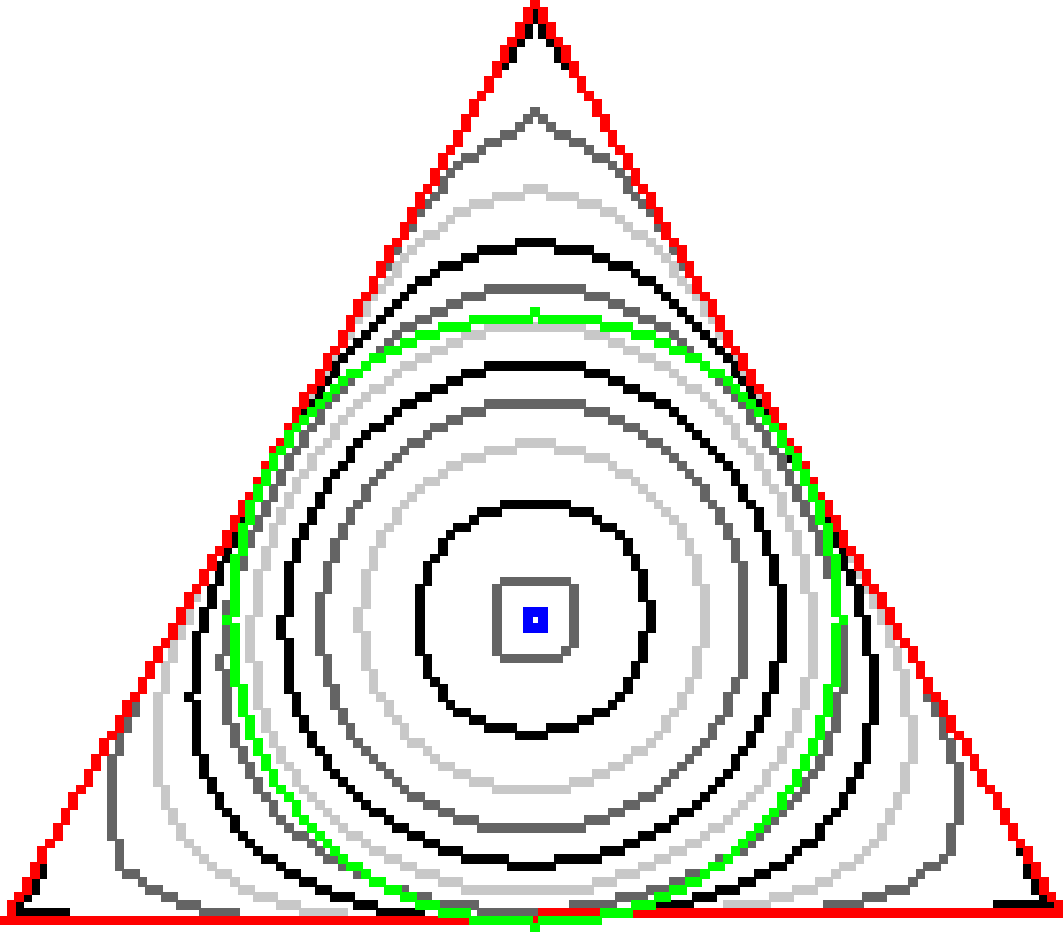
\includegraphics[scale=0.25]{figures/chapter8/graph-flow/triangle/neigh-0/alpha-0.01/summary.pdf} & 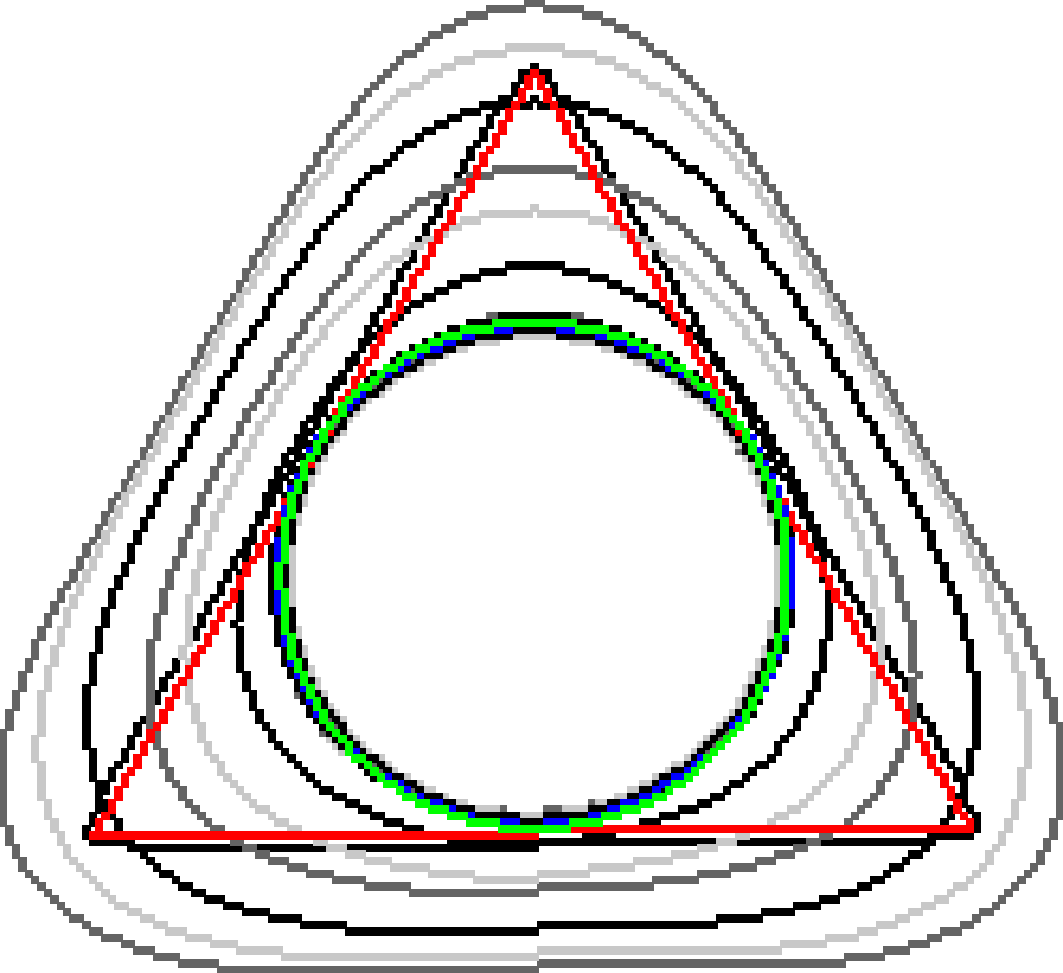
\includegraphics[scale=0.25]{figures/chapter8/graph-flow/triangle/neigh-2/alpha-0.01/summary.pdf} & 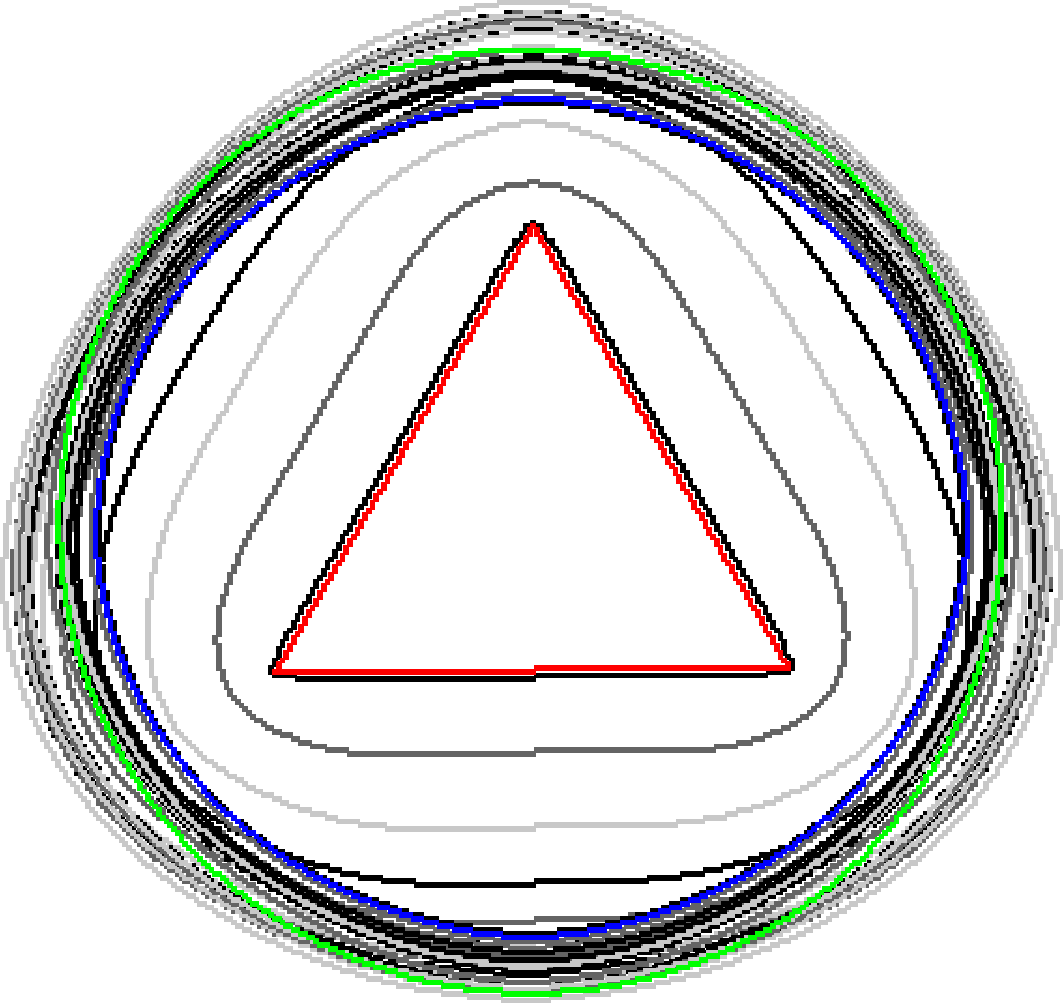
\includegraphics[scale=0.25]{figures/chapter8/graph-flow/triangle/neigh-2/alpha-0.001/summary.pdf}\\
$(n=2, a=0,\alpha=0.01)$ & $(n=2, a=2,\alpha=0.01)$ & $(n=2, a=2, \alpha=0.001)$
\end{tabular}}

\subfloat[$(n=2, a=2, \alpha=0.001)$]{
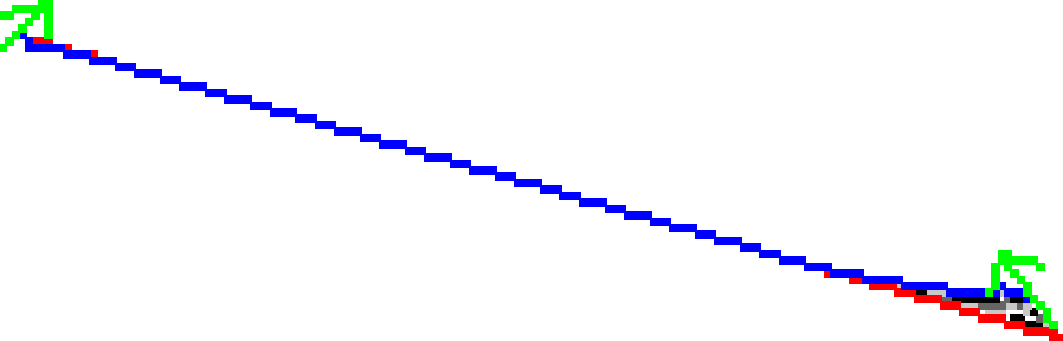
\includegraphics[scale=0.4]{figures/chapter8/constrained-elastica/curve-3/lp-0.001/summary.pdf}
}

\caption{\daniel{\textbf{GraphFlow results.}} The GraphFlow algorithm can shrink and grow in accordance with length penalization and it converges to a shape closer to the global optimum (green curve) in the free elastica problem. In the constrained elastica, we believe that we can improve the results by using a larger, possibly random, neighborhood. We are using $n=2,a=2$ and shapes are displayed at every $10$ iterations.}
\label{ch8:fig:graph-flow-neigh2-results}
\end{figure}

%\section{Injecting data term}
%
%The GrabCut model (see~\cref{app:grabcut-model}) is the state-of-art graph-based technique for image segmentation tasks . The GrabCut model possesses two data term components, one related to the boundary, and another to the region. Several works tried to inject geometric information in a graph-cut framework for image segmentation. While some works were sucessfuly in injecting perimeter penalization, those that attempt to include curvature suffered from lack of precision, lack of theoretical guarantees and high running times. In this section we propose a model that advances in these two criterias.
%
%Let $I:\Omega \rightarrow [0,1]^3$ a color image. We define $I(O_m)$ as the subset of $I$ restricted to the optimization region $O_m$. Let $X_m = X(I(O_m))$ and $x$ a possible binary assignment. We recall the GrabCut minimization energy for given parameters $\Lambda=(\lambda_r, \lambda_b)$, image $I$ and labeling $x$.
%
%\begin{align*}
%	grabc_{\Lambda}(I,x) &= \lambda_r \sum_{p \in \Omega}{regional(I,x,p)} + \lambda_b \sum_{p,q \in \Omega}{boundary(I,x,p,q)}.
%\end{align*}
%
%To construct the graph $G(\mathcal{V},\mathcal{E})$, we define the edge's weight function $w$ such that curvature and data terms are contemplated. Therefore,  
%
%\[
%	\forall p,q \in O_m, \quad w(v_p,v_q) = \left\{ \begin{array}{ll}
%		\beta(u(\Ds,p) + u(\Ds,q)) + \lambda_b boundary(I,x,p,q), & \text{if } p,q \notin T	\\
%		\beta M + \lambda_r regional(I,x,p,q), & \text{if } p \in T \text{ xor } q \in T \\
%		0, & \text{otherwise}
%	\end{array},\right.
%\]
%
%The validation function is defined as
%
%\begin{align*}
%val_{(\vec{\theta},\Lambda)}(\Ds^{(k-1)},I,x^{(k-1)}) &= \hat{E}_{\vec{\theta}}(\Ds) + grabc_{\Lambda}(I,x)
%\end{align*}
%
%Finally, the squared curvature correction algorithm is described as
%
%\begin{algorithm}
% \SetKwData{It}{k}
% \SetKwData{MIt}{maxIt}
% \SetKwData{Delta}{delta}
% \SetKwData{Tol}{tolerance}
% \SetKwInOut{Input}{input}\SetKwInOut{Output}{output}
% \SetKwComment{comment}{//}{}
% 
% \Input{A digital set $\Ds$; the optimization band $m$; the neighborhood explorer set size $a$;  parameter vector $\vec{\theta}=(\alpha,\beta)$; data term coefficients $\Lambda=(\lambda_r,\lambda_b)$; tolerance $tolerance$.}
% \BlankLine
% $\Ds^{(0)} \longleftarrow \Ds$\;
% $k \longleftarrow 1$\;
% \Delta $\longleftarrow +\infty$\;
% \While{ \It $<$ \MIt \bf{and} \Delta $>$ \Tol  }{ 	
%	$candidates \longleftarrow \{\}$\;
%	\comment{Candidate selection}
% 	\ForEach{ $X \in N_a(\Ds^{(k)})$ }
% 	{
% 		$candidates \longleftarrow candidates \cup x\big( \; \{ p \; | \; v_p \in C_s( X ) \} \; \big)$\;
% 	}
%
%	\comment{Candidate validation}
%	$\Ds^{(k)} \longleftarrow \displaystyle \argmin_{x \in candidates}{ val_{(\vec{\theta},\Lambda)}(\Ds^{(k-1)},I,x^{(k-1)})}$\; 	
%	\It $\longleftarrow$ \It $+1$\;
%	\Delta $\longleftarrow | val_{(\vec{\theta},\Lambda)}(\Ds^{(k)},I,x^{(k)}) - val_{(\vec{\theta},\Lambda)}(\Ds^{(k-1)},I,x^{(k-1)}) |$\;
%	
% }
% \caption{LSGF squared curvature segmentation correction algorithm.}
% \label{ch8:alglegc-segmentation-algorithm}  
%\end{algorithm}


\begin{figure}
\center
\begin{tabular}{cccc}
\multirow{2}{*}{Seeds} & \multirow{2}{*}{Graph cut} & $\alpha=0.05, \boldsymbol{\beta=0},$ & $\alpha=0.05, \boldsymbol{\beta=0.5},$\\
& & $\gamma_r=\gamma_b=1.0$ & $\gamma_r=\gamma_b=1.0$\\
 	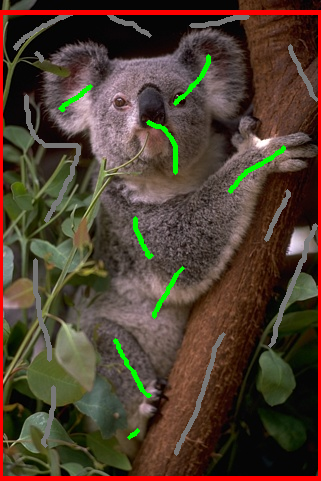
\includegraphics[scale=0.25]{figures/chapter8/segmentation/coala/k-0.0/seeds.png} & 
 	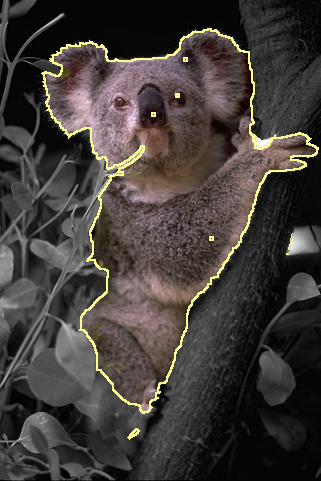
\includegraphics[scale=0.25]{figures/chapter8/segmentation/coala/k-0.0/gc-seg.png} &  	
 	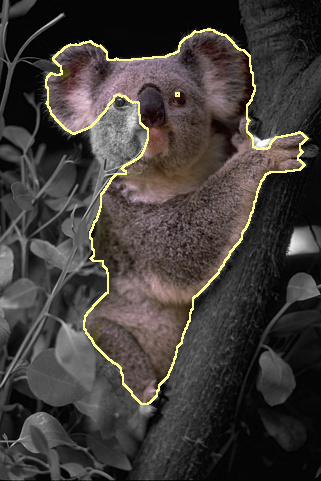
\includegraphics[scale=0.25]{figures/chapter8/segmentation/coala/k-0.0/corrected-seg.png} &  	
 	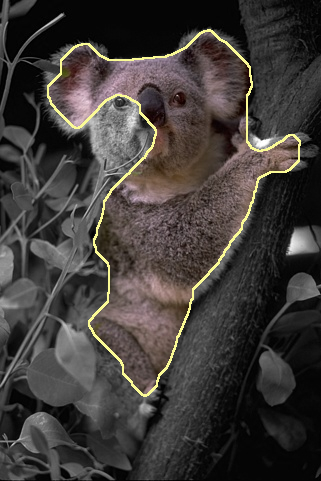
\includegraphics[scale=0.25]{figures/chapter8/segmentation/coala/k-0.5/corrected-seg.png}
\end{tabular}	
\caption{\daniel{\textbf{GraphFlow segmentation.}} Given foreground (green) and background (gray) seeds at picture (a); Graph cut produces picture (b) which is used as input of the GraphFlow algorithm; in pictures (c) and (d) we display the output of GraphFlow algorithm with and without squared curvature regularization. }
\label{ch8:fig:segmentation}
\end{figure}

\begin{figure}
\center
\begin{tabular}{cc}
$\alpha=0, \boldsymbol{\beta=0}$ & $\alpha=0, \boldsymbol{\beta=1}$\\
$\gamma_r = 3, \gamma_b = 3$ & $\gamma_r = 3, \gamma_b = 3$\\
 	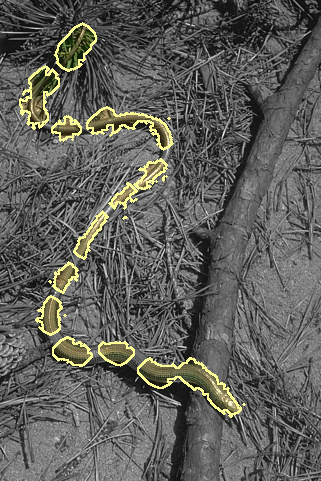
\includegraphics[scale=0.25]{figures/chapter8/completion/graphseg/alpha-0.0/beta-0.0/gamma-3.0/radius-7/corrected-seg.png} & 
 	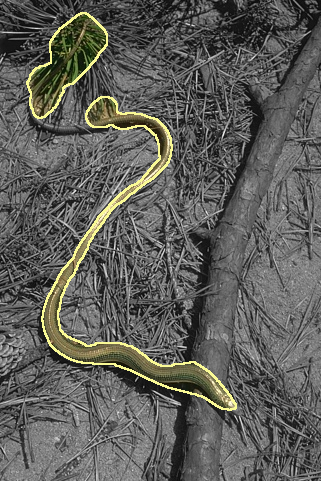
\includegraphics[scale=0.25]{figures/chapter8/completion/graphseg/alpha-0.0/beta-1.0/gamma-3.0/radius-7/corrected-seg.png}
\end{tabular}	
\caption{\daniel{\textbf{GraphFlow and completion property}}. The oversegmentation picture in the left was obtained with no squared curvature regularization, while the picture in the right was obtained by setting $\beta=1.0$. }
\label{ch8:fig:segmentation-curvature-completion}
\end{figure}

\section{Conclusion}
We described a graph cut model that regularizes the squared curvature and it is suitable for image segmentation. The evolution produced by the GraphFlow responds to the length penalization term $\alpha$, i.e., the shape tends to grow (shrink) for lower (higher) values of $\alpha$ and we observe a convergence to a shape closer to the global optimum in the free elastica problem. In the constrained elastica, we believe that a larger neighborhood is necessary to produce better results.  Finally, the GraphFlow~\cref{ch8:alg:graphflow-algorithm} is faster and simpler to implement than the previous models presented in this thesis.
